\documentclass[12pt]{article}

\usepackage{geometry}
 \geometry{
 a4paper,
 left=25mm,
 right=20mm,
 top=20mm,
 }
 
\usepackage{hyperref}
\usepackage{exercise}
\usepackage{enumerate}
\usepackage{graphicx}
\usepackage{subfig}
\usepackage{listings}

\usepackage{amsmath}
\usepackage{amsfonts}


\graphicspath{ {images/} }

\lstset{language=python, firstline=37, lastline=45, title={Listing 1: Data structures for cellular automaton}}

\begin{document}

\title{
Computational Geometry and Digital Images \\
\textbf{fork-recognition}\\
Project report
}

\author{Etienne Moutot, Ievgeniia Oshurko}
\date{April 6, 2016}
\maketitle


\section{Introduction}  

There is a great interest in a problem of shape matching and shape recognition \cite{Zhang20041}. We propose a solution to this problem based on Machine Learning techniques applied to global shape descriptors.

To build a global shape descriptor which would capture geometry and topology of the shapes in a given class various contour-based and region-based features were assembled into a global bag-of-features.

We test this approach in the provided dataset that consists of $1 050$ images from $70$ different classes.

The following Python tools were used on a different stages of project:
\begin{itemize}
\item Library \texttt{scikit-image} for image processing purposes \url{http://scikit-image.org/}
\item Couple of utils were used from computer vision library \texttt{mahotas} \url{http://mahotas.readthedocs.org/en/latest/} (such as hit\&miss, thinning algorithms).
\item Library \texttt{scikit-learn} for machine learning and data preprocessing \url{http://scikit-learn.org/}
\end{itemize}

\subsection{How to run our scripts}
First, you need \href{https://www.continuum.io/downloads}{\textbf{Anaconda}} to be installed on your computer.

Then, run the script \texttt{install\_dependencies.sh}, which will use pip to install all missing dependencies.

After that, compile the binary utilities needed for the scripts:\\
\texttt{cd bin}\\
\texttt{cmake -DDGtal\_DIR=YOUR\_DGTAL\_DIR}\\
\texttt{make}

\bigskip

Now, you have several python scripts available.

\textbf{We recommend to run the quick version of the scripts}. The behavior is the same, but the quick version does not computes "slow" features. Results are quite better with the slow version, but execution time is very long, so it is not very usable for large database. Moreover, the quick version stays very strong on classification.

\paragraph{distance.py} Usage: \texttt{python3 distance.py img1.pgm img2.pgm}

This script computes the distance between the two pictures. It is simply the $l_2$ norm of the difference of the feature vectors of the images (see below for the precise definition of these features).

The 3 Robustness scripts are modified to execute this distance script.

\paragraph{class.py, quick\_class.py}
Usage: \texttt{python3 quick\_class.py img.pgm}

This script outputs the probability of \texttt{img.pgm} to be in each class. 

To do so, it uses a classification model, which is trained using data stored into \texttt{X\_quick} and \texttt{y\_quick} files (\texttt{X} and \texttt{y} for slow version. 
Note that to run \textit{class.py}, you will to perform the learning by yourself !). These files are provided to you, but you can re-generate them using the script below.

The scripts \texttt{scriptClassification.sh} and \texttt{scriptQuickClassification.sh} are modified to use this classifier.

\paragraph{learn.py, quick\_learn.py}
Usage: \texttt{python3 quick\_learn.py}

This script generates the files \texttt{X\_quick} and \texttt{y\_quick} (or \texttt{X} and \texttt{y}) from a database stored into the directory \texttt{database/}.
These files contains all the features extracted from the images of the directory \texttt{database/}. It is useful to store them in order to not extract these features each time you want to use the classifier (this is quite long, even for the quick version).
All images from \texttt{database/} are used for the learning when you run this script !

Normally you don't have to run this script, unless you want to run the slow version, or try the script to be sure it works.

\section{Feature Engineering}

The extracted features capture the properties of shape: its topology and its geometry. In total, 38 features were developed:

\begin{itemize}
	\item Histogram of distance of the medial axis points from borders (\textbf{10 features} corresponding to 10 bins of histogram)
	\item Histogram of border curvature coefficients(\textbf{5 features} corresponding to 5 bins of histogram)
	\item Scaled area
	\item Solidity
	\item Extend
	\item Scaled major axis length
	\item Scaled minor axis length
	\item Histogram of medial axis straight lines length (\textbf{5 features} corresponding to 5 bins of histogram)
	\item Number of branches of medial axis skeleton
	\item Number of branched points of medial axis skeleton
	\item Scaled centroid displacement
	\item Asymmetry measures (\textbf{9 features} corresponding to horizontal and vertical flips, and rotation for 7 distinct angles)
\end{itemize} 

\subsection{Image preprocessing}
The images are pre-processed before we extract the features from them. There are three reasons for that:
\begin{itemize}
	\item We want to remove the noise from the image, because our features need to be robust to noise.
        \item We also want to remove the black holes that appears in some images.
        \item We want the shape to be white and the background black (one of the rats is reversed).
\end{itemize}

For that we implemented 3 transformations:
\begin{description}
	\item[Image padding]: The border of the image are just filled with a border of black pixels, in order to avoid problems when the shapes touch the border.
        \item[Shape filling]: The background is detected by the fact that it is the first connected component. Then it is filled in black and the rest of the image (the main shape) is filled with white. With that we remove all the wholes in the image.
        \item[Smoothing]: The goal of this smoothing is to get rid of the noise at the border of the shape. We apply to the image a median filter, with as neighbourhood a disk of a 7px diameter. After few tests, 7px seems to be a good compromise between smoothing and not loosing too much details. \\
        A median filter is a local filter which, for each pixel, replaces its colour by the colour of the median pixel in some shape around it (here a disk).
        
        \begin{figure}[h]
          \begin{center}
            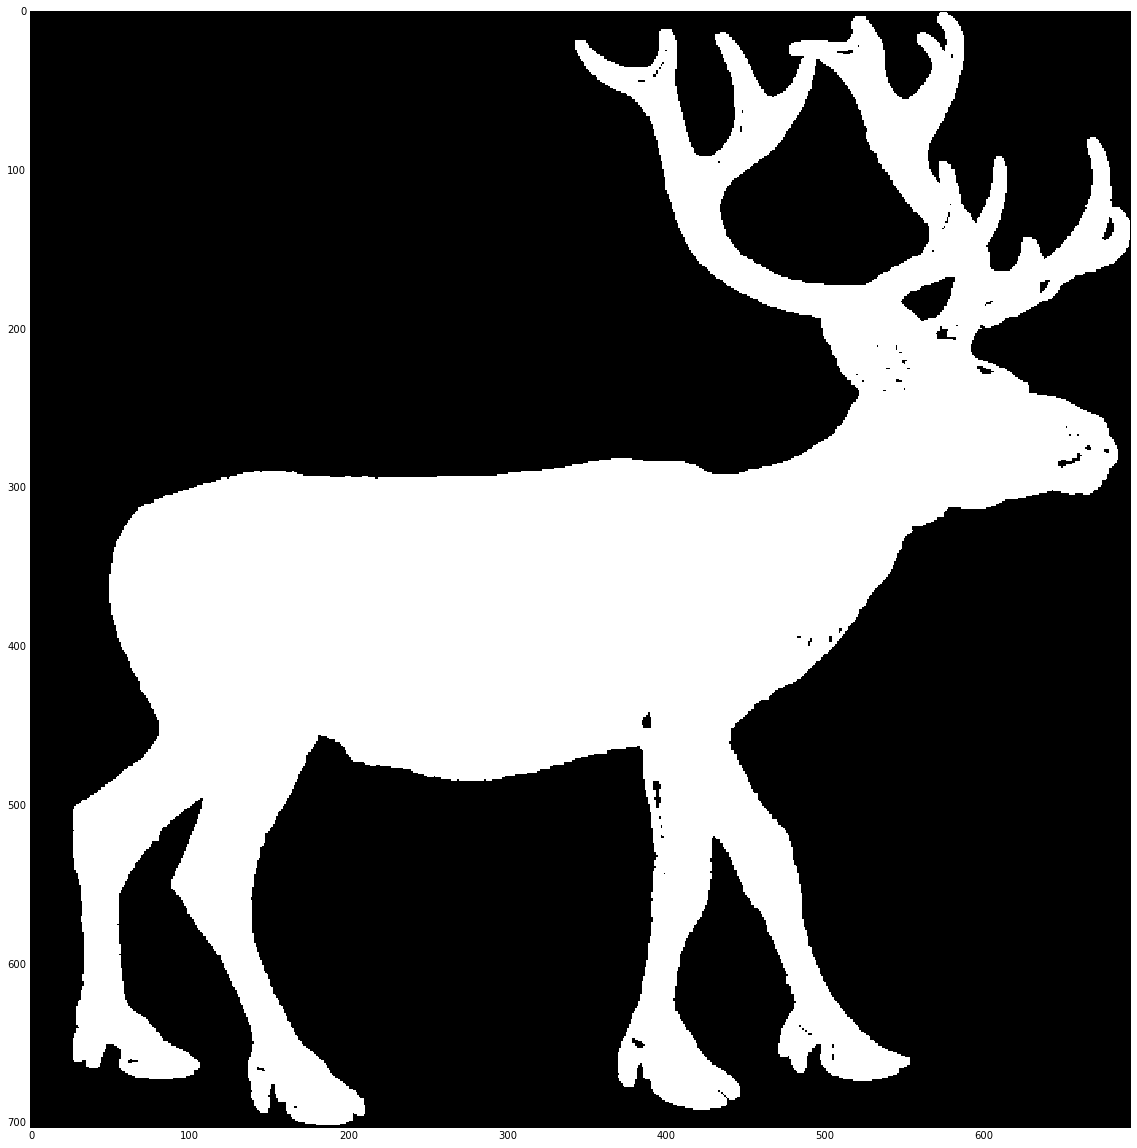
\includegraphics[scale=0.20]{deer_no_processing.png}
            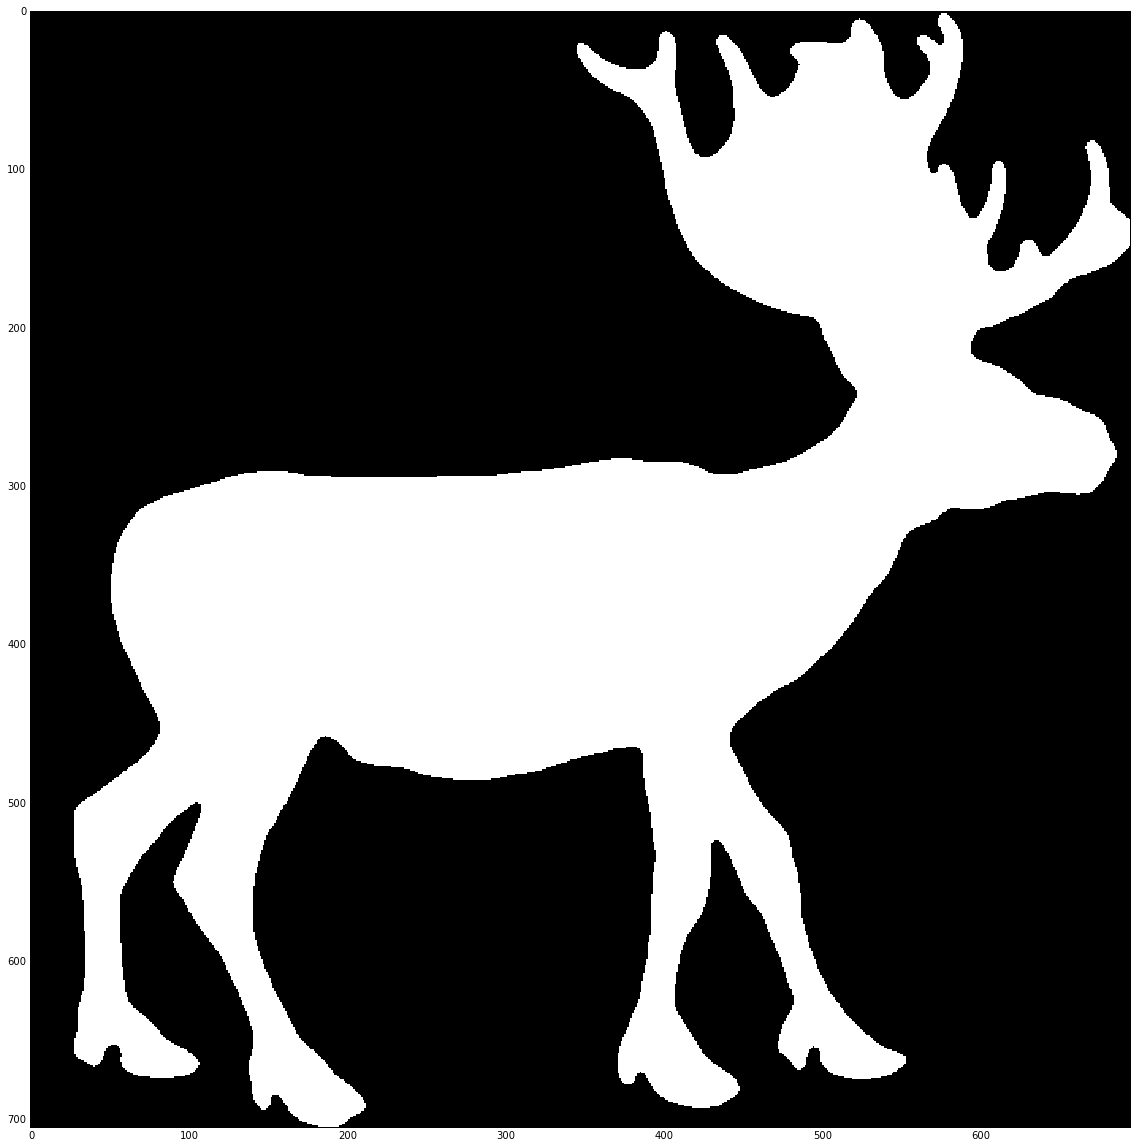
\includegraphics[scale=0.20]{deer_with_processing.png}
            \caption{Example without and with pre-processing}
          \end{center}
        \end{figure}
\end{description}

\subsection{Medial Axis}
We first generate the medial axis skeleton. The scikit implementation \cite{medial_axis} follows what was done in the lecture, adding an information to each point $p$: its distance to the border $d(p)$. This distance could also be seen as the radius of the maximal incircle with center $p$.

Then we try to extract some numerical features from this skeleton, which are all made to be scale-invariant (all features from skeleton are naturally rotation-invariant).

Skeletons of some shapes are illustrated by the figures below:

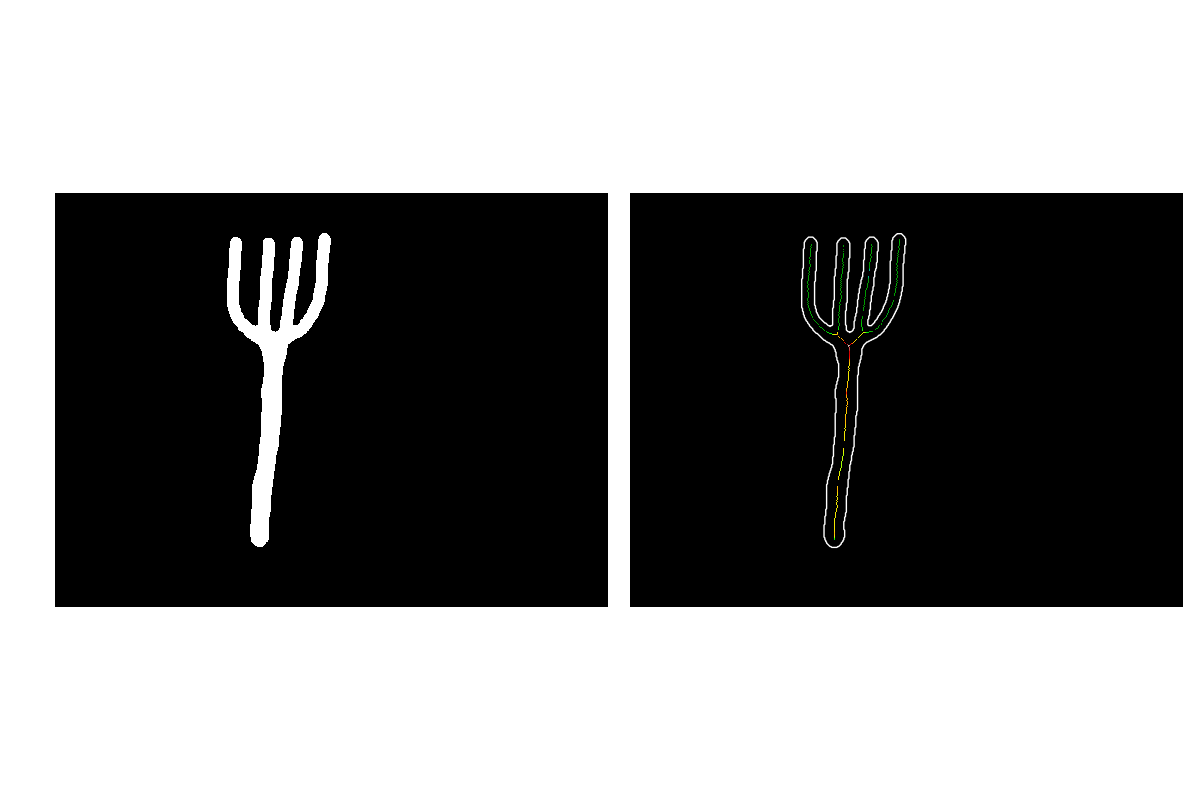
\includegraphics[scale=0.25]{fork_75.png}
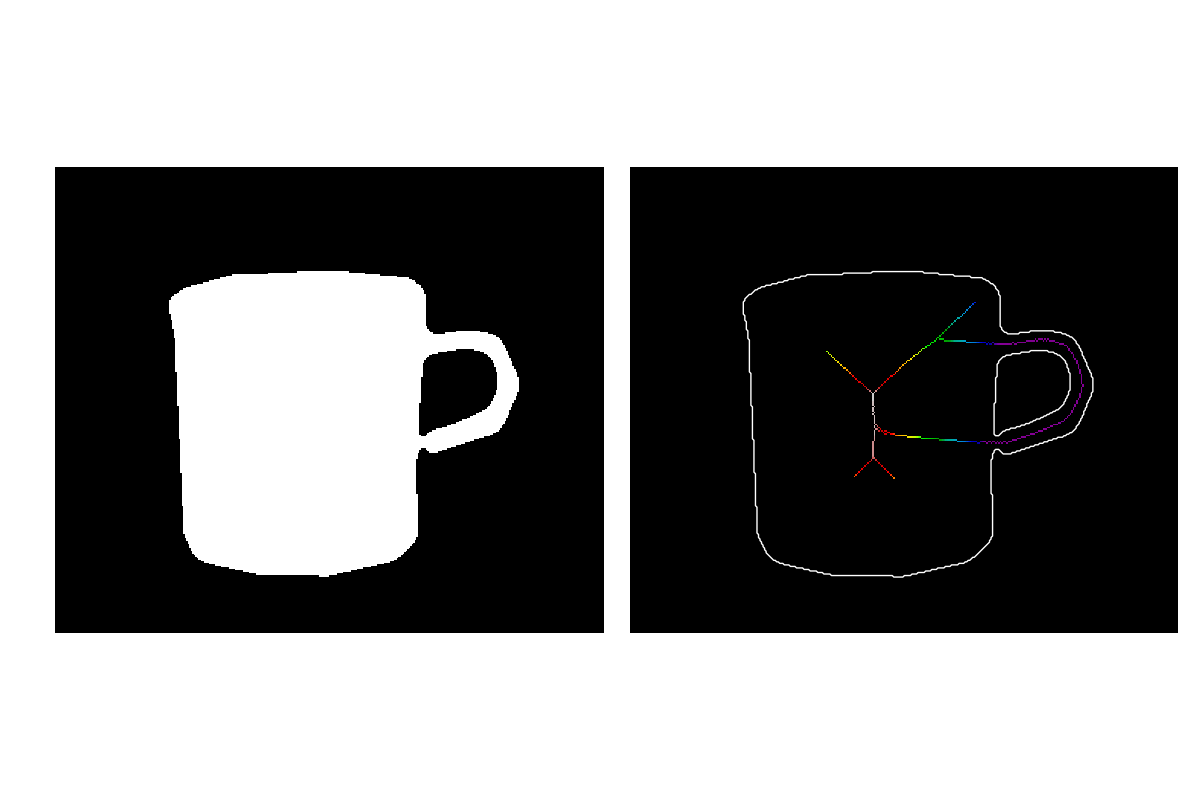
\includegraphics[scale=0.25]{cup_476.png}

\vspace{12px}

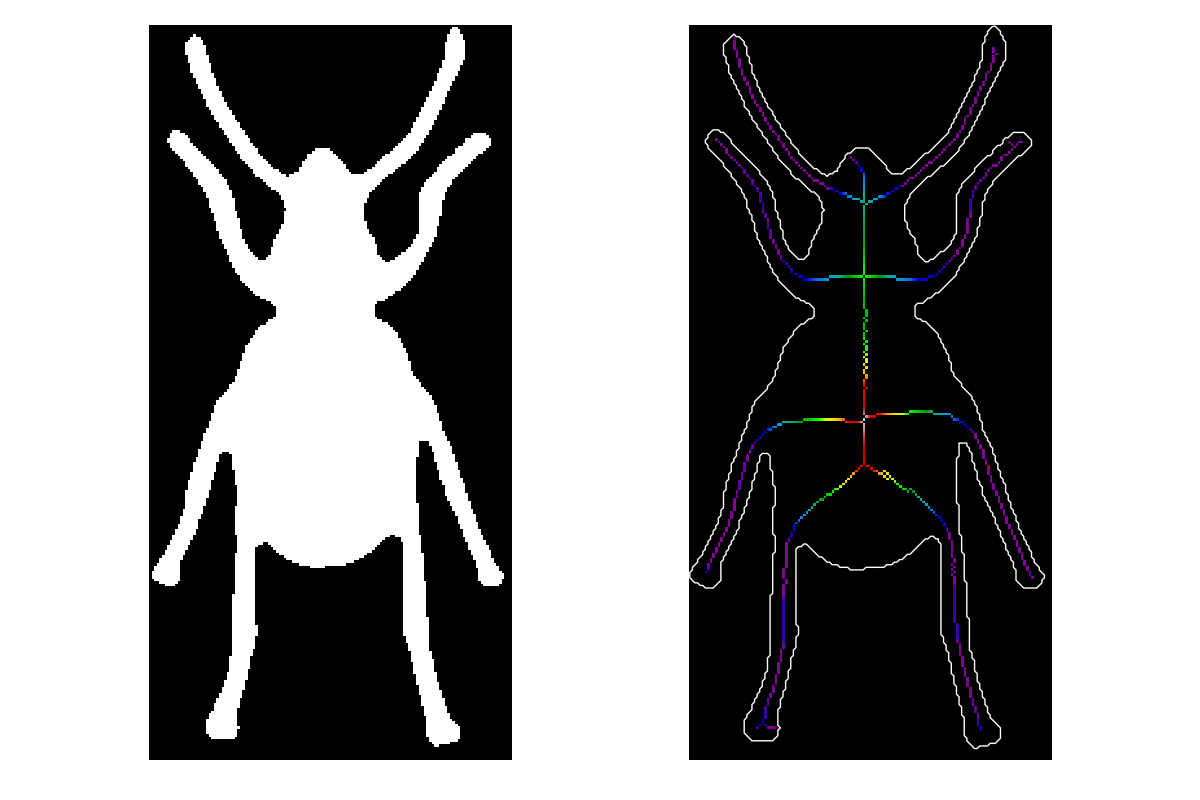
\includegraphics[scale=0.25]{beetle_281.png}
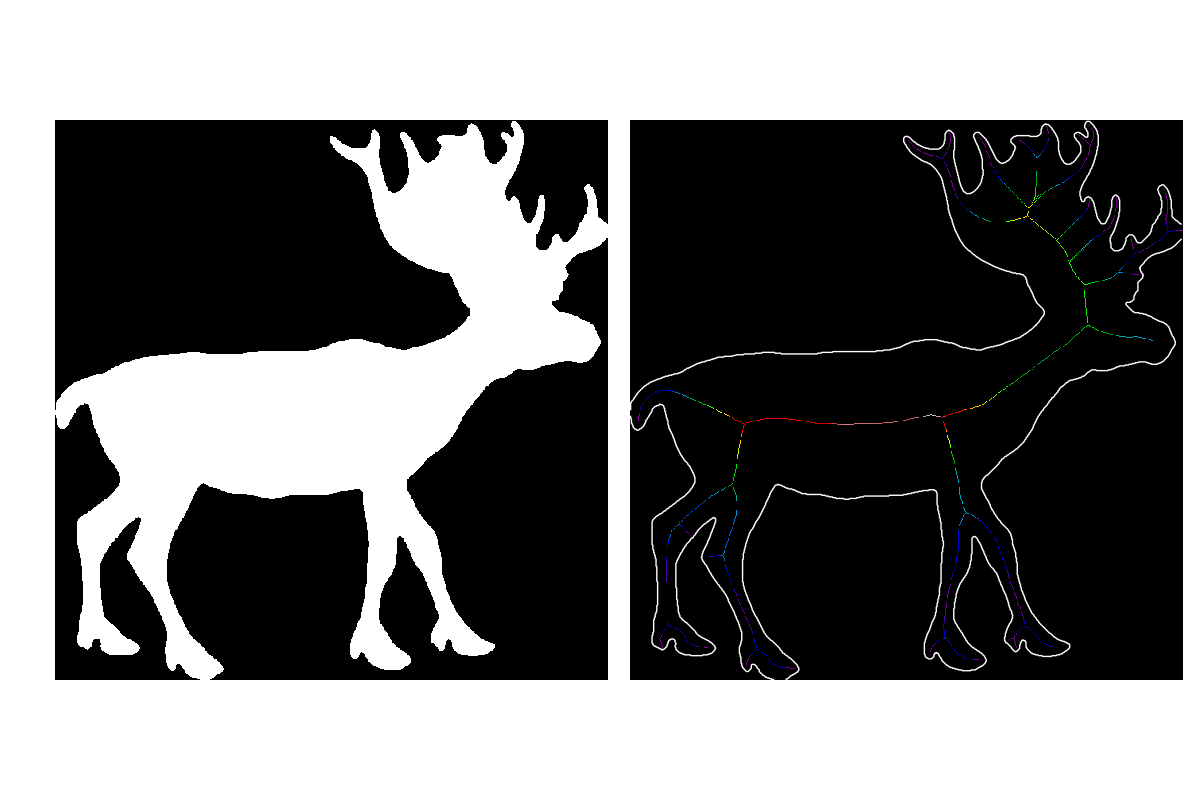
\includegraphics[scale=0.25]{deer_79.png}

\subsubsection{Histogram of distance of the medial axis points from borders}

The distance $d(p)$ characterizes the local thickness of the shape at the point $p$ of the skeleton. Thus our first feature is an histogram of the distances along the skeleton.

This histogram is cut into 10 bins, which are all normalized to be scale-invariant (only \textbf{the proportion} of pixels in each bins count instead of \textbf{the number} of pixels).

\subsubsection{Medial axis straight lines}
The second feature we propose is to decompose the skeleton into straight lines, ans the build an histogram of the size of the straights lines.
The idea of this feature is that the sizes of the straight lines tend to indicate if the object is "straight" or "curved", indeed if it is curved, there will be no long straight lines in its skeleton.

We make this feature scale-invariant by, again, normalizing the histogram obtained (divided into 5 bins).

Python implementation (\texttt{skimage.transform.probabilistic\_hough\_line}) of \textit{Probabilistic Hough Transform} \cite{Kiryati} was used to do this. \\
In this method, a straight line is represented by the segment perpendicular to it, parametrized by a pair $(\rho, \theta)$, where $\rho$ is a length of segment, and $\theta$ is an angle. \\
Hought transform consists of two steps: 
\begin{itemize}
  \item Parameter's plane of $(\rho, \theta)$ is divided into discrete grid (by parameter histogram bins). The array representing this grid contains number of pixels which are the closest to the respective line.
  \item An exhaustive search of the parameters with maximum frequency is performed. Each time a pixel close to a particular parametrized line is found, the corresponding value is incremented in the array.\\
  This step is called \textit{incremental step}, it usually dominates the execution time of Hough transform.
\end{itemize}

The increment of the array's value for a given pair of parameters is called voting, and the Probabilistic Hough Transform makes an assumption that it is enough for a random subset of image pixel to vote to find the maximum frequency parameters. So for our dataset experimentally we have choosen to detect the lines, for which numer of pixels voting for the pair of parameters is more than 10 (threshold value $T=10$).

Detecting the straight lines of our medial axis skeleton helps us to capture its geometry. Images below illustrate the result of straight lines detection on some examples from our dataset.

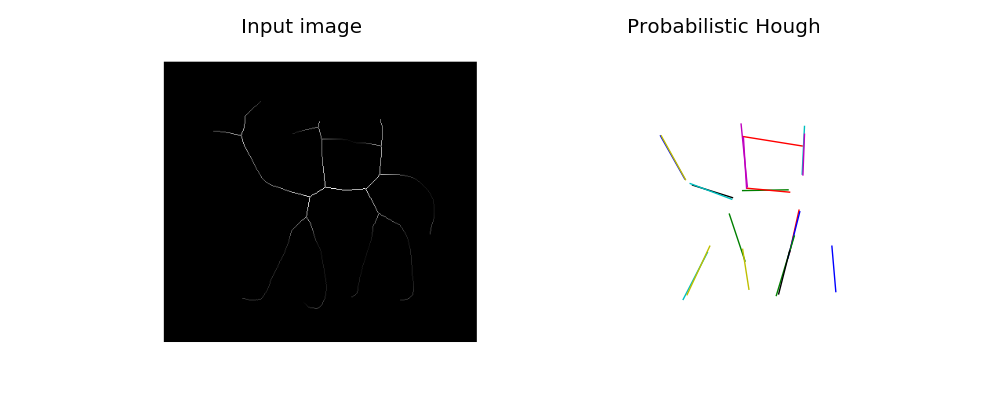
\includegraphics[scale=0.6]{camel_764.png}
\vspace{12px}

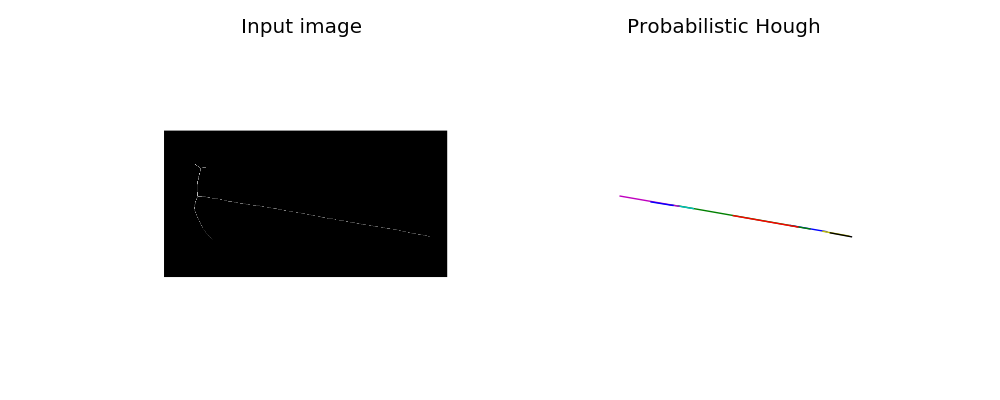
\includegraphics[scale=0.6]{hammer_604.png}

We have used as a subset of our features the histogram (5 bins) of the lengths of the detected straight lines, which characterizes the distribution of straight elements of medial axis skeleton for the given image.

\subsubsection{Quantitative features of skeleton}
We also extract some quantitative features from skeletons: number of branches and number of branched points (points of skeleton where the branches start).

These features are not normalized because they are already scale-invariant.

To find end-points of branches and branched points of skeleton we use the \texttt{mahotas.hitmiss} implementation of \textit{Hit and Miss Transform Algorithm}.

We provide to the algorithm all possible structures of the neighborhood of an end point (or respectively branched point) to recognise, for example:

\begin{center}
 	\begin{tabular}{| c | c | c |}
 		\hline
		0 & 0 & 0 \\ \hline
		0 & 1 & 0 \\ \hline
		2 & 1 & 2 \\ \hline
	\end{tabular}
\end{center}

where value 1 represents pixel that belongs to skeleton, 0 one that does not, and 2 represents that in this position we do not care whether the pixel belongs or not to the skeleton. This structure will match our end-point. We form 8 such possible structures for recognition of end-points of skeleton branches. The figure below illustrates an example of a matching structure for the branched point:
 
\begin{center}
 	\begin{tabular}{| c | c | c |}
 		\hline
			1 & 2 & 1 \\ \hline
			2 & 1 & 2 \\ \hline
			1 & 2 & 2 \\ \hline
	\end{tabular}
\end{center}


\subsection{Volumetric Features}
We also extract some features about the global shape.

\subsubsection{Scaled area}
We are interested in a feature representing the area of the object. The problem is that the surface of the shape is note a scale-invariant variable.

To solve this, our feature is:
$$\frac{\text{surface}}{\text{perimeter}^2}$$
which is scale-invariant (if the size is multiplied by $x$, the surface is multiplied by $x^2$ and so for $\text{perimeter}^2$).

\subsubsection{Solidity and extend}
\subsubsection{Scaled major and minor axes length}
\subsubsection{Scaled centroid displacement}

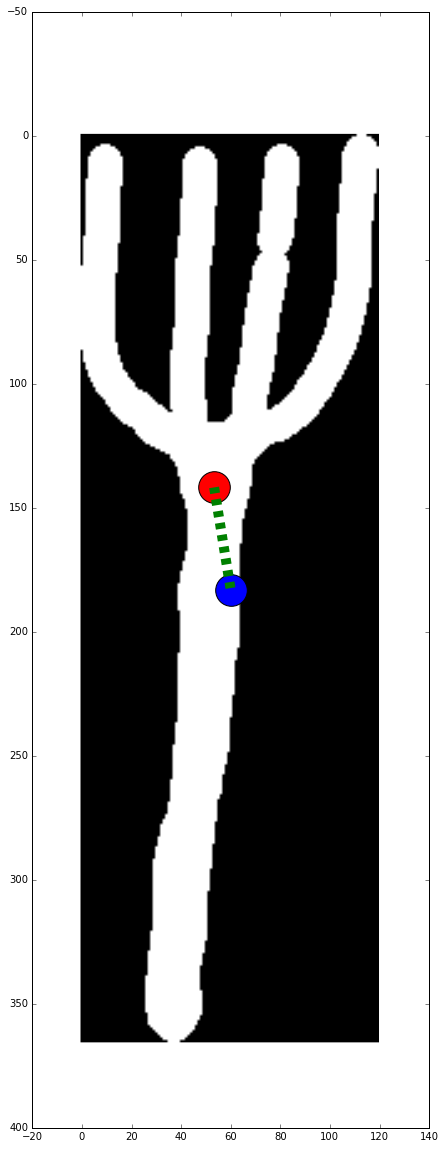
\includegraphics[scale=0.26]{fork_centroid.png}
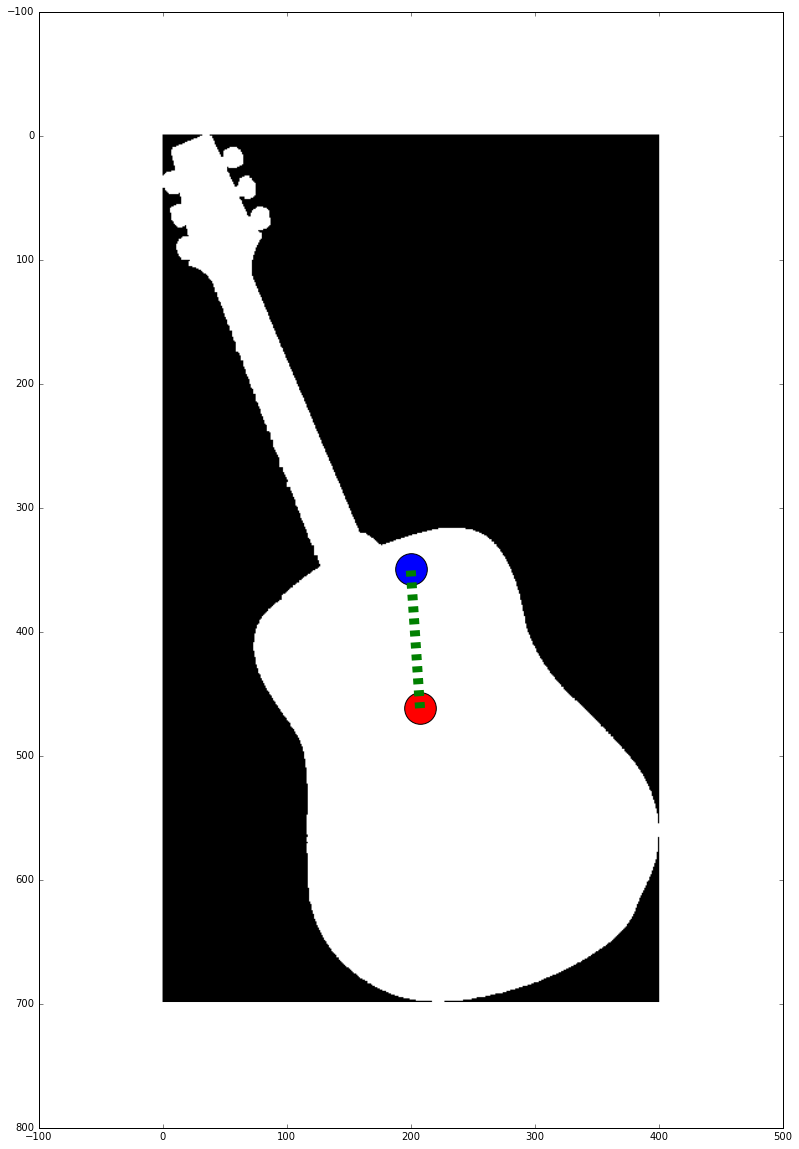
\includegraphics[scale=0.26]{guitar_centroid.png}
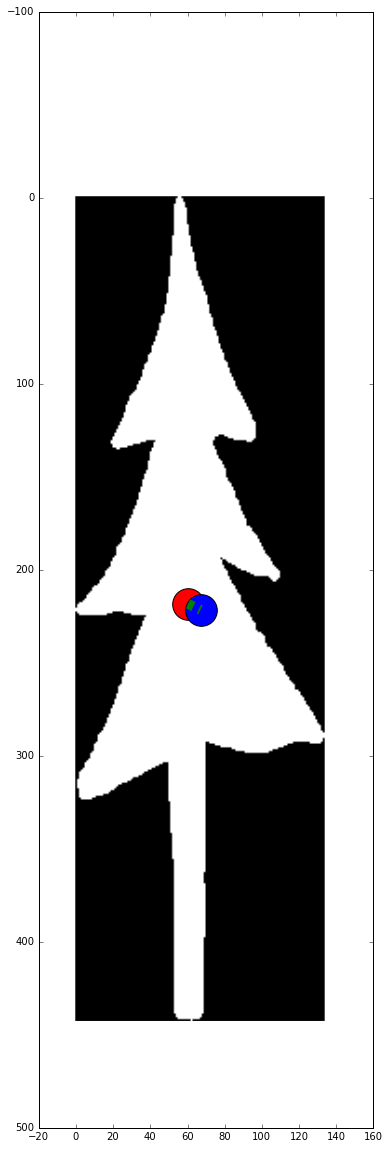
\includegraphics[scale=0.26]{tree_centroid.png}

\subsection{Asymmetry measures}
Distances from original image to its horizontal and vertical flips, to rotations for $k*\frac{\pi}{4}$
 
\section{Classification models}

Machine Learning techniques were used to build the model of shape recognition.  

\textit{Gaussian Naive Bayes Classifier}. Naive Bayes \cite{Bayes} is a supervised classification method which is based on Bayes' theorem and makes an assumption that the features are pairwise independent:

\begin{equation}
	P(y|x_{1} ... x_{n}) = \frac{P(y)P(x_{1} ... x_{n}|y)}{P(x_{1} ... x_{n})}
\end{equation}

Here $x_{1} ... x_{n}$ is a feature vector, and $y$ is the class label. Our features are continuous, so we use Gaussian modification of Naive Bayes that assumes that the likelyhood of a feature follows the normal distribution.

\textit{K-Nearest Neighbors Classifier}\cite{neighb}. To assign the class label this method uses a simple majority vote of the $k$ nearest neighbours to the provided sample. To find $k$ nearest neighbors different distance metrics may be used (we use standard Euclidean metric). 

Choice of the number of neighbours $k$ that take a part in voting for class assignment is highly dependent on data (larger $k$ reduces noise, but make the classification boundaries less strict). So, we have chosen to take values of $k=5$ and $k=20$ neighbours to analyse the classifation results on our dataset.

We used \texttt{sklearn.neighbors.KNeighborsClassifier()} implementation of K-Nearest Neighbors Classifier.
 
\textit{Support Vector Machines Classifier (SVM)} \cite{svm}. This machine learning method finds a separation hyperplane for the points in the given dataset, and tries to find this hyperplane is such a way that the distance between training set points and hyperplane is maximised. 

Depending on the kernel chosen for the SVM model (in our case we try two kernels: linear $\langle x, x'\rangle$ and radial basis function $\exp(-\gamma |x-x'|^2)$), the values of two paramaters need to be chose: $C$ and $\gamma$.



 The gamma parameters can be seen as the inverse of the radius of influence of samples selected by the model as support vectors.

The C parameter trades off misclassification of training examples against simplicity of the decision surface. A low C makes the decision surface smooth, while a high C aims at classifying all training examples correctly by giving the model freedom to select more samples as support vectors.



Two kinds of test were performed on the training dataset:
\begin{itemize}
	\item \textbf{Score out of one} class which represents the accuracy score (number of samples with correctly assigned classes over all given samples).
	\item \textbf{Score out of ten} most probable classes which represents the number of samples for which the correct class was found in 10 most probable classes over all given samples.
\end{itemize}

\begin{center}
  \begin{tabular}{| l | c | c |}
    \hline
    \textbf{Classifier} & \textbf{Score out of one} & \textbf{Score out of ten}\\ \hline \hline
    Gaussian Naive Bayes & 0.81 & 0.97 \\ \hline
	K-Nearest Neighbours (5 neighbours) & 0.71 & 0.95\\ \hline
	K-Nearest Neighbours (20 neighbours) & 0.60 & 0.98 \\ \hline
	SVM Classifier (linear kernel, C=1) & 0.76 & 0.93 \\ \hline
	\textit{SVM Classifier (RBF kernel, C=10, gamma=0.1)} & \textit{0.85} & \textit{0.98} \\ 
	\hline
  \end{tabular}
\end{center}

Parameters for SVM classifiers were chosen using the grid search according to the best score.

The following plot illustrates, in general, the confusion matrix between our classes and shows that for some classes classifier predicts more accurately then for others:

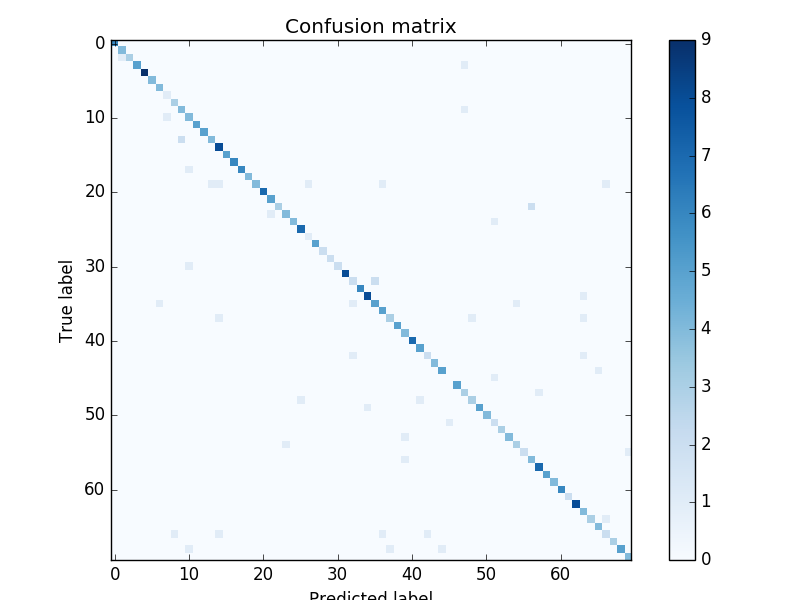
\includegraphics[scale=0.6]{confusion_matrix.png} 

The figures below are a part of more scaled version of confusion matrix, where we can see, for example, that for some \textit{"device"} classes the accuracy is very high and for others vise versa. Figure on the right shows us that in some cases the classifier confuses between shapes of a class \textit{"fork"} and ones of a class \textit{"spring"}, as well as \textit{"frog"} and \textit{"teddy"}.   

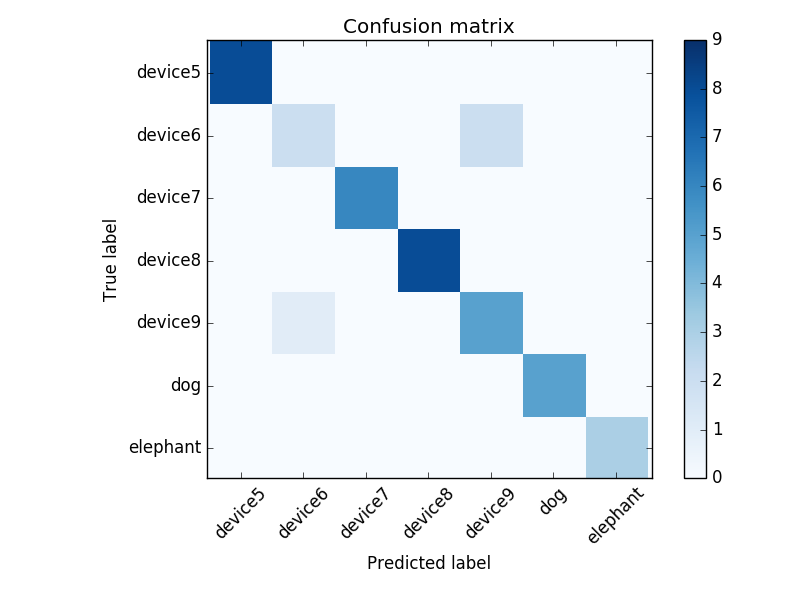
\includegraphics[scale=0.4]{device.png} 
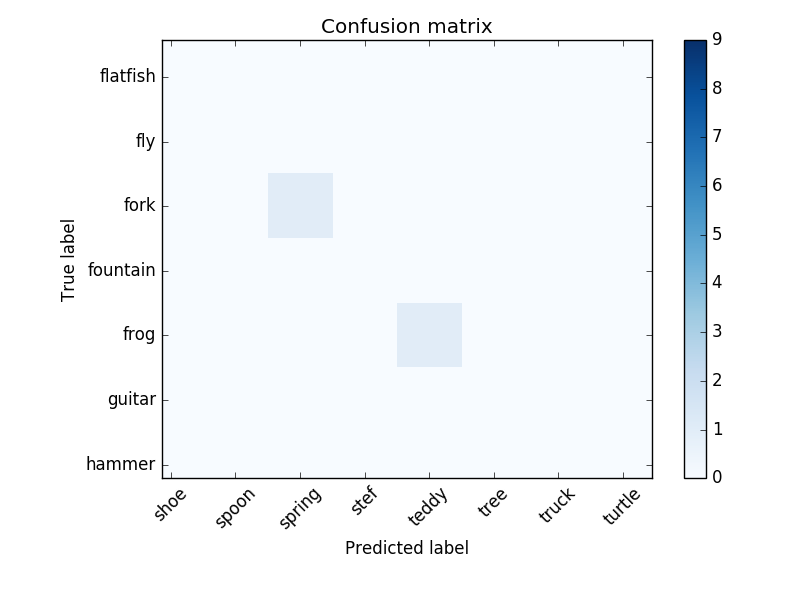
\includegraphics[scale=0.4]{fork_fish.png} 

\section{Discussions}
Presented above feature vector is normalized and can be used as a shape descriptor  

\subsection{Performance}
\subsection{Robustness and scale/rotation invariance}

\bibliographystyle{plain}
\bibliography{biblio}

\end{document}
